\documentclass[a4paper]{IEEEtran}
\usepackage[latin1]{inputenc}
\usepackage{epstopdf}
%\usepackage[spanish]{babel}
\usepackage[cmex10]{amsmath}
\interdisplaylinepenalty=2500
\usepackage{amsfonts}
\usepackage{amssymb}
\usepackage{graphicx}
\usepackage{verbatim}
\usepackage{array}
\usepackage{multirow}
\usepackage{dcolumn}
\usepackage{color}
\usepackage[noadjust]{cite}
\usepackage{url}
\usepackage{balance}
\usepackage[usenames,dvipsnames]{xcolor}
\DeclareGraphicsExtensions{.eps}

\DeclareMathOperator*{\Max}{max}
\DeclareMathOperator*{\Min}{min}
\DeclareMathOperator*{\argmin}{arg\,min}
\DeclareMathOperator*{\Maximize}{Maximize}

\begin{document}
\title{A non-parametric quantile autoregressive model for wind power Firm Energy Certificate}

\author{Henrique~Hoeltgebaum,
		Marcelo~Ruas,
		Cristiano~Fernandes
	    and Alexandre~Street,~\IEEEmembership{Member,~IEEE}

\thanks{This work was partially supported by the R\&D project ANEEL PD-7625-0001/2013.}
\thanks{Henrique Hoeltgebaum, Marcelo Ruas, Cristiano Fernandes and Alexandre Street are with the Electrical Engineering Department, Pontifical Catholic University of Rio de Janeiro (PUC-Rio), Rio de Janeiro, RJ, Brazil (e-mail: \mbox{hhhelfer@hotmail.com}; \mbox{mcruas@gmail.com}; \mbox{cris@ele.puc-rio.br}; \mbox{street@ele.puc-rio.br}).}
}

\maketitle
\begin{abstract}
	In this article we use the framework of a non-parametric quantile regression model to generate forecasts of wind capacity factors of several quantiles. Such scenarios are then used as input to raise the distribution of the quantiles associated with each wind plant. In our proposed model we introduce a $\ell_{1}$ penalty term in the objective function, in order to properly adress an adaptive dependency structure for the $\alpha$-quantile time series. Hence, in contrast to the well-known quantile regression model, our proposed framework is not limited to linear functions. Computation experiments show a slight improvement when comparing our non-parametric framework to the benchmark.
		
%	In this article we use the framework of a non-parametric quantile regression model to generate forecasts of wind capacity factors of several quantiles. Such scenarios are then used as input to raise the distribution of the quantiles associated with each wind plant. In our proposed model we introduce a $\ell_{1}$ penalty term in the objective function, in order to properly adress an adaptive dependency structure for the $\alpha$-quantile time series. Hence, in contrast to the well-known quantile regression model, our proposed framework is not limited to linear functions. Computation experiments show a slight improvement when comparing our non-parametric framework to the benchmark.  	


\end{abstract}

\begin{IEEEkeywords}
	Quantile regression, quantile autoregressive models, firm energy certificate, wind power, $\ell_{1}$-penalty term, time varying quantiles.
\end{IEEEkeywords}

% ===== Sec. I - Introduction ===== %

\section{Introduction}
\IEEEPARstart{W}{i}nd Firm Energy Certificate (FEC) estimation impose several challenges. First and foremost, it is a quantile function of an aleatory quantity, named here on wind capacity factor (WP). Due to its non-dispachable profile, accurate scenario generation model could reproduce a fairly dependence structure in order to the estimation of FEC. Secondly, as a quantile function, the more close to the extremes, more sensitive to sampling error.

In this work, we introduce a new non-parametric quantile autoregressive model with $\ell_{1}$-penalty term, in order to properly simulate FEC densities for several $\alpha$-quantiles. 


\subsection{Review of the Brazilian Electricty Sector}
In response to the growing demand of energy, Brazil began a period of major structural reforms in the 1990s \cite{portal13}. Such reforms were positively accepted by private investors, which leads to numerous concession auctions for new projects \cite{barroso06}. Such enviroment had a mood turn over during 2001-2002, since the former security criteria were fully based on market mechanism and lead to a serious supply crisis. The outcomes of such crisis were the reduction of total load by 20\% and an economic loss of tens of billions US dollars \cite{pereira04}.

Therefore, as a response to aforementioned crisis, brazilian government developed a new power sector model in 2004 \cite{barroso06}. The implementation of the reformed framework for Brazil's electricity sector generally aims to provide the long-term system's expansion incentive, reduce uncertainty in generation companies future revenues, and mitigate unfavourable effects of the short-term market \cite{street09}.

In addition, such system was applied to the Brazilian case based on mandatory reability contracts as an incentive to investors. These contracts are considered to be financial instruments, in the same spirit as forward contracts. Moreover, in order to provide a confidence sensibility over generation, all contracts ought to be covered by so-called ``firm energy certificates'' (FEC). These FECs are defined in GWh/year and represent the plant's physical energy production capacity. In a nutshell, the FEC of a certain plant is the maximum amount of energy that can be sold through contracts and establishes the reliability assured by the generator backing the contract. It is thus a critical parameter for the power plant's economic feasibility.

\subsection{Motivation and objetives}
Accurate estimation of FEC values provide the investors safety regarding his cash-flows, since the main issue about introducing renewable energy into energy matrixes is its intermitent\footnote{When there is no human intervention over its production.} profile. Regarding wind power, its production is fully conditioned to the wind speed, which is caused by diference in atmospheric pressure. Hence, prior knowledge over its future behaviour is essential when considering the generation of this renewable source.

Regarding wind plants, its FEC where fully detailed on a document produced by ANEEL in July of 2008 [XXX], which defines the firm energy certificate of a wind plant as the mean of the monthly production. As described in the mentioned document, the estimation of wind plants FEC is given by

\begin{equation} 
FEC^{(\alpha)} =\sum_{m=1}^{12} \frac{E_m^{(\alpha)} \times h_m}{8760}, \label{eq:FEC}
\end{equation}					
\noindent
where $FEC^{(\alpha)}$ denotes the FEC of the wind plant certified with $\alpha$\% of confidence, ${h_m}$ is the number of hours in the month ${m}$ and $E_m^{(\alpha)}$ denotes the mean of the monthly quantiles certified at $\alpha$\%. In practice, the generator provides 12 values of energy certified at $\alpha$\%. refering to the month $m$. 

To give the reader a further understanding about Equation \eqref{eq:FEC}, we present in Figure \ref{percentiles_FEC} the calculated FEC's for a windplant located at the brazilian northeast, named Icaraizinho. The estimatives $E_m^{(\alpha)}$ for several $\alpha \in \{50,55,...,95\}$ are ploted.

%O critério P50% indica que em 50% dos anos do histórico utilizado, a energia produzida em um determinado mês m superou o valor E_m^((50%)). Quando aumentamos o critério de confiabilidade de 50% para um valor α > 50, esperamos ver uma redução da GF. Os dois gráficos que são exibidos a seguir mostram, para um parque no Nordeste do Brasil (Icaraizinho), as estimativas E_m^((α%)) e GF^((α%)) para diversos valores de confiabilidade α∈{50,55,…,95}.

\begin{figure}[H]
\centering
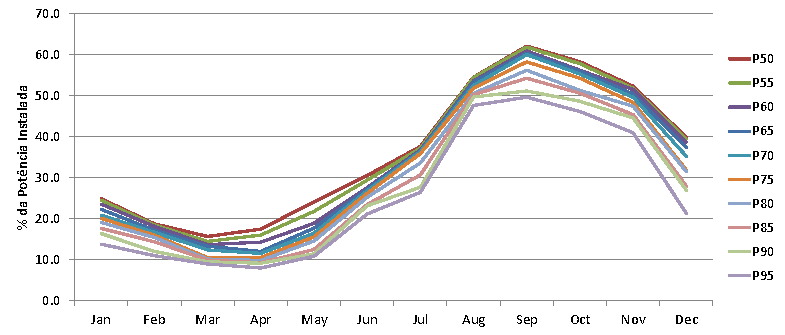
\includegraphics[height=3.5cm,width=7cm]{Figures/GF_SIM.pdf}
\caption{Percentiles $E_m^{(\alpha)}$ for each month $m$ and confidence criteria $\alpha$.}
\label{percentiles_FEC}
\end{figure}


%Onde $GF^{(\alpha)}$ representa a Garantia Física da usina em questão certificada a um nível $\alpha$\% de confiança, ${h_m}$ é o número de horas no mês ${m}$ e $E_m^{(\alpha)}$ denota a média dos quantis mensais certificados a $\alpha$\%, i.e., recebe-se um conjunto de 12 valores de energia certificados a $\alpha\%$ referentes ao mês \emph{m}. Logo, a GF de uma usina é assumida ser uma variável aleatória, uma vez que está em função da produção da usina, pois ($E_m^{(\alpha)}$) é calculado com base no histórico do fator de capacidade da usina e este depende unicamente da produção da mesma, que por definição é uma variável estocástica.
%
%O cálculo alternativo proposto por esta dissertação é utilizar o \emph{quantil das médias mensais} dos cenários ao invés das \emph{médias dos quantis mensais}. Através disso, o novo cálculo para a garantia física tomaria a seguinte forma, esboçado pela equação \eqref{eq:3}.
%\vspace{-1pt}
%\begin{align} 
%	\begin{split}
%	GF_{alternativa}^{(\alpha)} =\mathbb{Q}^{(\alpha)}\Bigr( \sum_{i=1}^{31} \sum_{m=1}^{12} \frac{{\tilde{G}}_{m,i}^ \times h_m}{8760}\Bigl) \label{eq:3}
%	\end{split}					
%\end{align}
%
%Onde $\mathbb{Q}^{(\alpha)}$ representa o quantil de $\alpha\%$, ${\tilde{G}}_{m,i}$ representa a geração média do cenário simulado do mês $m$ do ano $i$ e $h_m$ o número de horas do mês $m$, compondo assim uma média de geração ponderada pelo número de meses.

 
% Figura XX - COLOCAR A GERAÇÃO EÓLICA AQUI
%
%Devido à essa característica, o novo marco regulatório estabelece que, para usinas com perfil de geração intermitêntes, a respectiva produção de cada uma dessas usinas deve estar assegurada por um Certificado de Garantia Física (GF) expedido pela ANEEL. Ou seja, as usinas geradoras devem emitir, atrelada à sua produção, um valor (em MW médio) que representa a quantidade máxima de energia que esta pode se comprometer a comercializar sob condições adversas, a um certo nível de probabilidade $\alpha$, ao longo do ano. Para usinas hidroelétricas, por exemplo, esses valores representam a capacidade da usina de produzir energia em períodos (anos) secos \cite{faria09}.
%
%Esses valores também figuram como responsáveis pela expansão segura da oferta, pois os mesmos agregam um certo nível de confiança aos contratos, dado que 100\% da carga de todas as Distribuidoras devem ser cobertas por contratos futuros assegurados pela GF de cada unidade geradora, i.e., as geradoras podem comercializar um valor menor ou igual à soma das GF's individuais das usinas contratadas. Criando assim um ambiente favorável à novos investimentos em geração reduzindo a incerteza a cerca dos possíveis \emph{déficits} de produção.
%
%A importância em calcular com precisão esse valor, para a geradora, se materializa no momento da entrega da energia, dado que contratualmente sua produção atual de energia será medida e comparada com a GF da usina. Assim, em adição ao risco de liquidação no mercado de curto prazo, o investidor fica sujeito a penalidades regulatórias se a produção de energia verificada ficar abaixo dos valores declarados, pois qualquer desvio é penalizado a um preço que reflete o custo de energia nova. Já para a distribuidora, esse valor é visto como balizador para a escolha de usinas contratadas por disponibilidade.  Contratos atrelados a usinas certificadas a um maior nível de confiança ($\alpha$), irão gerar uma receita maior e mais frequente à curto prazo através da liquidação do \emph{surplus} de energia no mercado \emph{spot}. 
%
%Um sistema certificado, a um maior nível de comprometimento de entrega, contará com um \emph{surplus} de energia para o atendimento à demanda maior e mais frequente. Além de Consumidores e Investidores, o Operador Nacional do Sistema (ONS) também se beneficia sob um maior nível de confiabilidade de entrega de energia, pois reduzirá assim o risco das usinas não atenderem suas respectivas demandas, causando um racionamento. Entretanto, como tudo que possui maior valor deve custar mais caro, os preços de \emph{breakeven} de empreendimentos eólicos deverão acompanhar o aumento da confiabilidade de forma a compensar a redução de GF, uma vez que ao aumentarmos o nível de confiabilidade $\alpha$ o valor de GF é reduzido. Assim, existe um claro \emph{tradeoff} entre o aumento da qualidade da energia para o sistema e o aumento de preço que poderá ser oferecido nos leilões por esses empreendimentos. Uma das motivações dessa dissertação é medir esse potencial impacto no preço dos empreendimentos eólicos no âmbito do ACR. 
%
%% COLOCAR O GRÁFICO AQUI QUE TÁ NA NOTA TÉCNICA? PROBLEMA É QUE TEREMOS QUE EXPLICAR DE ONDE VEM OS DADOS E TAL...
%
%Na prática, o cálculo da GF de uma usina eólica necessita de uma série de dados (da produção histórica da usina) de tamanho significativa, de forma que a medida obtida possa ser confiável. Em se tratando de usinas eólicas no Brasil, a possibilidade de se obter séries com tamanhos adequados é bem restrita. As usinas mais antigas no país estão operando há no máximo dois anos. Portanto as séries de dados de velocidade de vento, pressão do ar e temperatura ambiente, registradas com rigor necessário para avaliação do potencial de energia eólica, ainda são relativamente pequenas. Isso impede a realização das simulações estocásticas de geração eólica, integrada ao sistema interligado hidrotérmico nacional, com o Modelo NEWAVE [\cite{street01}, \cite{portaria}]. Tais simulações são fundamentais para fomentar a confecção de estratégias de comercialização e investimento competitivas ao investidor. 
%
%É importante notar que sob o olhar dos financiadores de projeto, usinas eólicas certificadas a 90\% são mais atrativas perante as demais. Isso porque a razão social dos bancos financiadores não é a produção de energia, consequentemente esses não possuem uma estratégia para anular o risco de baixa performance dos parques. Por consequência, o financiador fica exposto ao risco de uma eventual inadimplência em caso de baixa performance dos parques e o mesmo não recebe nada a mais em caso de boa performance [NT street]. Posto que esse aumento de confiabilidade é de suma importancia para agentes financiadores, esse trabalho se propõe a estudar a questão do erro amostral atrelada à essa estimativa. Pois o cálculo da GF leva em consideração o percentil da produção anual, esse percentil é uma estatística de ordem e o erro amostral gerado pela sua estimação fica sujeito a um aumento, ao elevarmos o nível de confiança $\alpha$ \cite{casella}. Como já citado anteriormente, o tamanho das séries de energia eólica no país é limitado, logo, como os percentis são definidos por mês, o percentil de 90\%, contará com um número muito menor de dados observados do que no percentil de 50\%, expondo-o a um erro amostral na estimação do percentil extremo. A utilização indevida desse valor pode estar penalizando o investidor, pois este paga um valor mais elevado por uma energia que acredita estar sendo assegurada sob um maior nível de confiabilidade, como o 90\%, quando na realidade seu valor foi mal estimado e o investidor corre o risco de ter seu lastro de venda reduzido.








%%%%%%%%%%%%%%%%%%%%%%%%%%%%%%%%%%%%%%%%%%%%%%%%%%%%%%%%%%%%%%%%%%%

%A certificação de uma usina e a estipulação do montante de energia que esta pode comercializar é denominada de garantia física (GF). No contexto atual, o cálculo da garantia física de uma determinada usina eólica é realizado com base na média da produção mensal certificada. Essa energia certificada é determinada pelo percentil  $\alpha$\% ou $P(\alpha)\%$ da produção histórica de cada mês do ano. Com isso, o certificador entrega para o empreendedor, 12 valores correspondentes ao percentil empírico $\alpha$\% de cada mês em MW médio, de energia certificada a $P(\alpha)\%$. A $GF^{(\alpha\%)}$ é a média desses 12 valores, conforme especificada pela Equação \ref{eq:1}, e indica que em $\alpha$\% dos anos do histórico utilizado, a energia produzida em um determinado mês \emph{m} superou o valor do percentil $\alpha$\% da série histórica.  
%
%Assim, na prática o cálculo da GF de uma usina eólica necessita de uma série de dados (da produção histórica da usina) de tamanho significativa, de forma que a medida obtida possa ser confiável. Em se tratando de usinas eólicas no Brasil, a possibilidade de se obter séries com tamanhos adequados é bem restrita, uma vez que as usinas mais antigas no país estão operando há no máximo dois anos. Portanto as séries de dados de velocidade de vento, pressão do ar e temperatura ambiente, registradas com rigor necessário para avaliação do potencial de energia eólica ainda são relativamente pequenas. Isso impede a realização das simulações estocásticas de geração eólica, integrada ao sistema interligado hidrotérmico nacional, com o Modelo NEWAVE. Tais simulações são fundamentais para fomentar a confecção de estratégias de comercialização e investimento competitivas ao investidor. 
%
%Para suprimir essa restrição, utilizaremos uma metodologia desenvolvida para extender os históricos de velocidade de vento pelo uso de regressão multivariada. Assim, obteremos estimativas dos fatores de capacidade das usinas que utilizaremos para o cálculo de suas respectivas GF pelo uso das duas abordagens: (i) a corrente em uso e (ii) uma alternativa que será proposta.
%


  

%penetration of wind energy into electricity matrixes is growing fast worldwide. In 2008 the installed capacity of wind power exceeded 120.000 MW. Only in Brazil, an estimation of its production capacity spins around 140.000 MW \cite{porrua2010wind}. In order to properly management the electricity generation provided by this renewable source, suitable models ought to be proposed to generate accurate forecasts. 


% However, after a few short years, political and economic challenges swiftly altered the invest- ment climate for the worse. In particular, between 2001-2002 the reform’s pure reliance on market mechanisms to provide security of supply led to a serious supply crisis resulting in the necessary reduction of total load (base and peak) by 20% [45]. This, in turn, resulted in an economic loss of tens of billions of US dollars [45]. In response, in 2004 the government launched a new power sector model, introducting a second stage in the Brazilian power sector reform [7]. Learning from their mistakes, the new model maintained the positive apsects of the first reform, while introducing a mixed investment environment, with competition and private sector participation to build new capacity [7]. In particular, this second stage of reform has increased the importance of long-term signals in contract prices and dropped short-term spot prices due to the advantage of the former in terms of providing a degree of certainty in the generator’s cash flow, with demand coming from contract markets, rather than from the volatile and risky spot market [9].


%Desde 2009 a comercialização dessa fonte de energia no país se baseia em um mecanismo de leilões anuais \cite{street01}. Os leilões foram introduzidos após o marco regulatório estabelecido em Março de 2004 e detalhado em Julho do mesmo ano, neles são disponibilizados contratos bilaterais de longo-prazo de venda de energia elétrica. Isto é, as distribuidoras de energia participantes do leilão disputam lotes de energia oferecidos pelas geradoras a fim de garantir o abastecimento de suas respectivas demandas, após acordado o preço é estabelecido um contrato bilateral regulando os termos e condições de fornecimento.
%
%Esse marco regulatório foi consolidado pela Lei n.º 10.848/04 e regulamentado pelo Decreto nº 5.163/04 que, entre outros assuntos, criou dois ambientes de contratação de energia, o Ambiente de Contratação Livre (ACL) e o  Ambiente de Contratação Regulada (ACR). Os contratos oferecidos dentro do ACR são chamados de Contrato de Comercialização de Energia Elétrica no Ambiente Regulado (CCEEAR). Esses contratos são firmados através da utilização de dois instrumentos financeiros conhecidos, contratos futuro (contrato de quantidade) e opções (contrato por disponibilidade). Já no Ambiente de Contratação Livre (ACL) existe uma alta flexibilidade com relação à contratação e ainda incentivos para a contratação com fontes renováveis, como descontos referentes as tarifas de transmissão e distribuição (TUST/TUSD). Qualquer contrato de compra e venda firmado nesses ambientes, deve ser registrado na Câmara de Comercialização de Energia Elétrica (CCEE) \cite{ccee}, balizando assim a contabilização da liquidação das diferenças entre a quantidade de energia gerada e a quantidade de energia contratada no volátil mercado de curto prazo, que será discutido com maiores detalhes posteriormente.
%
%Esses contratos de longo-prazo figuram como os principais responsáveis pela expansão segura da oferta, uma vez que fornecem um sinal de preço mais adequado para os investidores no setor de geração em relação ao preço de curto prazo \cite{barroso06b}, pois reduzem a incerteza no fluxo de caixa da Geradora e mitiga o risco do mercado de energia de curto prazo. Essa segurança com relação ao fluxo de caixa do investidor é de fundamental importância, uma vez que o principal problema atrelado ao uso de fontes renováveis é o perfil inconstante de sua geração. Em se tratando de energia eólica, a produção de energia por parte do aerogerador, é função da disponibilidade dos ventos. %A Figura XX explicita o perfil altamente intermitente e sazonal da geração eólica para (DA ONDE VEM OS DADOS?).
%
%% Figura XX - COLOCAR A GERAÇÃO EÓLICA AQUI
%
%Devido à essa característica, o novo marco regulatório estabelece que, para usinas com perfil de geração intermitêntes, a respectiva produção de cada uma dessas usinas deve estar assegurada por um Certificado de Garantia Física (GF) expedido pela ANEEL. Ou seja, as usinas geradoras devem emitir, atrelada à sua produção, um valor (em MW médio) que representa a quantidade máxima de energia que esta pode se comprometer a comercializar sob condições adversas, a um certo nível de probabilidade $\alpha$, ao longo do ano. Para usinas hidroelétricas, por exemplo, esses valores representam a capacidade da usina de produzir energia em períodos (anos) secos \cite{faria09}.
%
%Esses valores também figuram como responsáveis pela expansão segura da oferta, pois os mesmos agregam um certo nível de confiança aos contratos, dado que 100\% da carga de todas as Distribuidoras devem ser cobertas por contratos futuros assegurados pela GF de cada unidade geradora, i.e., as geradoras podem comercializar um valor menor ou igual à soma das GF's individuais das usinas contratadas. Criando assim um ambiente favorável à novos investimentos em geração reduzindo a incerteza a cerca dos possíveis \emph{déficits} de produção.
%
%A importância em calcular com precisão esse valor, para a geradora, se materializa no momento da entrega da energia, dado que contratualmente sua produção atual de energia será medida e comparada com a GF da usina. Assim, em adição ao risco de liquidação no mercado de curto prazo, o investidor fica sujeito a penalidades regulatórias se a produção de energia verificada ficar abaixo dos valores declarados, pois qualquer desvio é penalizado a um preço que reflete o custo de energia nova. Já para a distribuidora, esse valor é visto como balizador para a escolha de usinas contratadas por disponibilidade.  Contratos atrelados a usinas certificadas a um maior nível de confiança ($\alpha$), irão gerar uma receita maior e mais frequente à curto prazo através da liquidação do \emph{surplus} de energia no mercado \emph{spot}. 
%
%Um sistema certificado, a um maior nível de comprometimento de entrega, contará com um \emph{surplus} de energia para o atendimento à demanda maior e mais frequente. Além de Consumidores e Investidores, o Operador Nacional do Sistema (ONS) também se beneficia sob um maior nível de confiabilidade de entrega de energia, pois reduzirá assim o risco das usinas não atenderem suas respectivas demandas, causando um racionamento. Entretanto, como tudo que possui maior valor deve custar mais caro, os preços de \emph{breakeven} de empreendimentos eólicos deverão acompanhar o aumento da confiabilidade de forma a compensar a redução de GF, uma vez que ao aumentarmos o nível de confiabilidade $\alpha$ o valor de GF é reduzido. Assim, existe um claro \emph{tradeoff} entre o aumento da qualidade da energia para o sistema e o aumento de preço que poderá ser oferecido nos leilões por esses empreendimentos. Uma das motivações dessa dissertação é medir esse potencial impacto no preço dos empreendimentos eólicos no âmbito do ACR. 
%
%% COLOCAR O GRÁFICO AQUI QUE TÁ NA NOTA TÉCNICA? PROBLEMA É QUE TEREMOS QUE EXPLICAR DE ONDE VEM OS DADOS E TAL...
%
%Na prática, o cálculo da GF de uma usina eólica necessita de uma série de dados (da produção histórica da usina) de tamanho significativa, de forma que a medida obtida possa ser confiável. Em se tratando de usinas eólicas no Brasil, a possibilidade de se obter séries com tamanhos adequados é bem restrita. As usinas mais antigas no país estão operando há no máximo dois anos. Portanto as séries de dados de velocidade de vento, pressão do ar e temperatura ambiente, registradas com rigor necessário para avaliação do potencial de energia eólica, ainda são relativamente pequenas. Isso impede a realização das simulações estocásticas de geração eólica, integrada ao sistema interligado hidrotérmico nacional, com o Modelo NEWAVE [\cite{street01}, \cite{portaria}]. Tais simulações são fundamentais para fomentar a confecção de estratégias de comercialização e investimento competitivas ao investidor. 
%
%É importante notar que sob o olhar dos financiadores de projeto, usinas eólicas certificadas a 90\% são mais atrativas perante as demais. Isso porque a razão social dos bancos financiadores não é a produção de energia, consequentemente esses não possuem uma estratégia para anular o risco de baixa performance dos parques. Por consequência, o financiador fica exposto ao risco de uma eventual inadimplência em caso de baixa performance dos parques e o mesmo não recebe nada a mais em caso de boa performance [NT street]. Posto que esse aumento de confiabilidade é de suma importancia para agentes financiadores, esse trabalho se propõe a estudar a questão do erro amostral atrelada à essa estimativa. Pois o cálculo da GF leva em consideração o percentil da produção anual, esse percentil é uma estatística de ordem e o erro amostral gerado pela sua estimação fica sujeito a um aumento, ao elevarmos o nível de confiança $\alpha$ \cite{casella}. Como já citado anteriormente, o tamanho das séries de energia eólica no país é limitado, logo, como os percentis são definidos por mês, o percentil de 90\%, contará com um número muito menor de dados observados do que no percentil de 50\%, expondo-o a um erro amostral na estimação do percentil extremo. A utilização indevida desse valor pode estar penalizando o investidor, pois este paga um valor mais elevado por uma energia que acredita estar sendo assegurada sob um maior nível de confiabilidade, como o 90\%, quando na realidade seu valor foi mal estimado e o investidor corre o risco de ter seu lastro de venda reduzido.


%%%%%OBJETIVOS

%A energia eólica é uma fonte inflexível, comparada às fontes hídricas e térmicas convencionais que possuem capacidade de reserva e podem gerenciar a sua operação, a qual conforme exposto na Seção \ref{sec:motivacao} possui um perfil intermitente não possuindo domínio sobre seus períodos de geração. Cientes das restrições na realização do cálculo da GF para empreendimentos de energia eólica, o objetivo principal dessa dissertação é estudar o cálculo desse importante parâmetro para o sistema, visando suprir as deficiências supracitadas da metodologia em uso. 
%
%Inicialmente, afim de dirimir o fato do erro amostral e obtermos resultados mais confiáveis para esse parâmetro, será abordada uma metodologia de extensão de históricos apresentada em \cite{streetEjoaquim} (que será posteriomente descrita com maiores detalhes). Obter-se-à séries de produção mais longas e assim, será possível uma melhor compreensão quanto aos percentis extremos, menos susetíveis ao erro amostral causado pelo aumento no nível de confiança no cálculo da GF. 
%
%Posteriormente, serão construídos intervalos de confiança não paramétricos para esses percentis. Com o intuito de verificar se, de fato, o cálculo em questão está expondo o investidor a uma redução de lastro em sua comercialização injustamente. Será levantada por simulação Monte Carlo uma distribuição multivariada de GF para determinados $\alpha$'s. Numa segunda etapa, ao invés de utilizar os percentis empíricos, estes podem ser obtidos a partir dos percentis de distribuições probabilísticas ajustadas às séries mensais de produção, como por exemplo Weibull, gama generalizada etc.  Em particular essas distribuições podem ser especificadas utilizando o arcabouço dos modelos \emph{Generalized Autoregressive Scores} (GAS) \cite{modeloGAS01}. É importante mostrar que o resultado do cálculo da metodologia vigente deve cair dentro dos intervalos de confiança dos estimadores que serão levantados. Ou seja, o ponto a ser comparado deve ser calculado com o histórico sob a metodologia e depois, os resultados confrontados com os ICs.



%%%%%%% GARANTIA FÍSICA
%\section{Garantia Física} \label{explic_GF}
%
%A certificação de uma usina e a estipulação do montante de energia que esta pode comercializar é denominada de garantia física (GF). No contexto atual, o cálculo da garantia física de uma determinada usina eólica é realizado com base na média da produção mensal certificada. Essa energia certificada é determinada pelo percentil  $\alpha$\% ou $P(\alpha)\%$ da produção histórica de cada mês do ano. Com isso, o certificador entrega para o empreendedor, 12 valores correspondentes ao percentil empírico $\alpha$\% de cada mês em MW médio, de energia certificada a $P(\alpha)\%$. A $GF^{(\alpha\%)}$ é a média desses 12 valores, conforme especificada pela Equação \ref{eq:1}, e indica que em $\alpha$\% dos anos do histórico utilizado, a energia produzida em um determinado mês \emph{m} superou o valor do percentil $\alpha$\% da série histórica.  
%
%Assim, na prática o cálculo da GF de uma usina eólica necessita de uma série de dados (da produção histórica da usina) de tamanho significativa, de forma que a medida obtida possa ser confiável. Em se tratando de usinas eólicas no Brasil, a possibilidade de se obter séries com tamanhos adequados é bem restrita, uma vez que as usinas mais antigas no país estão operando há no máximo dois anos. Portanto as séries de dados de velocidade de vento, pressão do ar e temperatura ambiente, registradas com rigor necessário para avaliação do potencial de energia eólica ainda são relativamente pequenas. Isso impede a realização das simulações estocásticas de geração eólica, integrada ao sistema interligado hidrotérmico nacional, com o Modelo NEWAVE. Tais simulações são fundamentais para fomentar a confecção de estratégias de comercialização e investimento competitivas ao investidor. 
%
%Para suprimir essa restrição, utilizaremos uma metodologia desenvolvida para extender os históricos de velocidade de vento pelo uso de regressão multivariada. Assim, obteremos estimativas dos fatores de capacidade das usinas que utilizaremos para o cálculo de suas respectivas GF pelo uso das duas abordagens: (i) a corrente em uso e (ii) uma alternativa que será proposta.
%
%Atualmente o cálculo da GF  dos empreendimentos de energia eólica, segundo a portaria ANEEL 258 de julho de 2008, é realizado com base na média da produção mensal de energia certificada. Conforme descrito na portaria, o cálculo consiste em:
%\vspace{-1pt}
%\begin{align} 
%	\begin{split}
%	GF^{(\alpha)} =\sum_{m=1}^{12} \frac{E_m^{(\alpha)} \times h_m}{8760} \label{eq:1}
%	\end{split}					
%\end{align}
%
%Onde $GF^{(\alpha)}$ representa a Garantia Física da usina em questão certificada a um nível $\alpha$\% de confiança, ${h_m}$ é o número de horas no mês ${m}$ e $E_m^{(\alpha)}$ denota a média dos quantis mensais certificados a $\alpha$\%, i.e., recebe-se um conjunto de 12 valores de energia certificados a $\alpha\%$ referentes ao mês \emph{m}. Logo, a GF de uma usina é assumida ser uma variável aleatória, uma vez que está em função da produção da usina, pois ($E_m^{(\alpha)}$) é calculado com base no histórico do fator de capacidade da usina e este depende unicamente da produção da mesma, que por definição é uma variável estocástica.
%
%O cálculo alternativo proposto por esta dissertação é utilizar o \emph{quantil das médias mensais} dos cenários ao invés das \emph{médias dos quantis mensais}. Através disso, o novo cálculo para a garantia física tomaria a seguinte forma, esboçado pela equação \eqref{eq:3}.
%\vspace{-1pt}
%\begin{align} 
%	\begin{split}
%	GF_{alternativa}^{(\alpha)} =\mathbb{Q}^{(\alpha)}\Bigr( \sum_{i=1}^{31} \sum_{m=1}^{12} \frac{{\tilde{G}}_{m,i}^ \times h_m}{8760}\Bigl) \label{eq:3}
%	\end{split}					
%\end{align}
%
%Onde $\mathbb{Q}^{(\alpha)}$ representa o quantil de $\alpha\%$, ${\tilde{G}}_{m,i}$ representa a geração média do cenário simulado do mês $m$ do ano $i$ e $h_m$ o número de horas do mês $m$, compondo assim uma média de geração ponderada pelo número de meses.


% ===== Sec. II - Parametric and Non-parametric models ===== %

\section{Parametric model}
Here we donoted as parametric model the well-known quantile regression model \cite{koenker2005quantile}. In contrast to the linear regression model through ordinary least squares (OLS), which provides only an estimation of the dependent variable conditional mean, quantile regression model yields a much more detailed information concerning the complex relationship about the dependent variable and its covariates, as defined by Equation \eqref{eq:QR}, 

\begin{equation} 
	\begin{split}
	\mathcal{Q}_{y}(\alpha|x_{1}, x_{2}, ..., x_{n}) = \beta_{0}(\alpha) + \beta_{1}(\alpha)x_{1} + \beta_{2}(\alpha)x_{2} + ...\\ + \beta_{n}(\alpha)x_{n} + \emph{F}^{-1}_\varepsilon(\alpha), \label{eq:QR}
	\end{split}					
\end{equation}
\noindent
where $\emph{F}_\varepsilon$ denotes the error density function.

\subsection{Parameter estimation}\label{QR_estimation}
The parameters of the quantile regression are estimated by a linear programming optimization problem that can be formulated as

\begin{equation} 
	\underset{\beta \; \in \; \mathbb{R}^{p} \times \mathbb{R}^{2n}_{+} }{\text{min}} \{\tau \mathbf{1}_{n}^{T}u + (1-\tau)\mathbf{1}_{n}^{T}v | X\beta + u - v = y \} .\label{PL}
\end{equation}

Here, $X$ stands for the usual covariates matrix, the residual vector $ y-X\beta $ splits itself into negative and positive parts ($u$ and $v$).


%{\parindent0pt onde $ X $ representa a matriz usual dos regressores n por p. Divide-se o vetor de resíduos $ y-X\beta $ em partes negativas e positivas ($u$ e $v$), e então estamos minimizando uma função linear em um poliedro restrito por um conjunto de restrições, e muitas das propriedades importantes das soluções, $\hat{\beta(\tau)}$, os quais são denominamos "quantis regressores", são derivadas imediatamente a partir de propriedades de soluções bem conhecidas de problemas lineares. }
%
%
%%%%%%%%%%%%%%%%%%%%%%%%%%%%%%%%%%%%%%%%%%%%%%%%%%%%%%%%%%%%%%%%%%%%%%%%%%%%%%%%%%%%%%%%%%%%%%%%%%%%%%%%%%%%%%%%%%%%%%%%%%%%%%%%%%%%%%%%%%%%%%%%%%%%%%%%%%%%%%%%%%%%%%%%%%%%
%\subsection{Seleção do modelo}
%Conforme apresentado na Seção 4.9.1 de \cite{koenker2005quantile}, existe uma vasta literatura a respeito de seleção de modelos. Serão abordados apenas alguns desenvolvimentos recentes a cerca do tema. 
%
%Em \cite{machado1993robust} é apresentada uma variação do critério de penalização de Schwarz para M-estimadores de regressão, incluindo o caso da regressão quantílica. É enfatiza a necessidade de procedimentos invariantes a locação e escala: para regressões da mediana ($\tau$=1/2) o seguinte cálculo rende o critério,
%\vspace{-10pt}
%\begin{align} 
%	\begin{split}
%	SIC(j) = log(\hat{\sigma}_{j})+\frac{1}{2}p_{j}\;log\;n,\label{eq:SIC}
%	\end{split}					
%\end{align}
%
%{\parindent0pt onde $\hat{\sigma}_{j}=\sum_{i=1}^{n} \rho_{1/2}(y_{i}-x^{T}_{i}\hat{\beta}_{n}(1/2))$ e $p_{j}$ indica a dimensão do $j$-ésimo modelo. Esse procedimento rende uma seleção de modelo consistente sob a circustância de que um dos modelos $p_{j}$-dimensional esteja de fato bem especificado.}
%
%Alternativamente ao critério supracitado, podemos considerar o critério de Akaike, calculado conforme
%\vspace{-10pt}
%\begin{align} 
%	\begin{split}
%	AIC(j) = log(\hat{\sigma}_{j})+p_{j}.\label{eq:AIC}
%	\end{split}					
%\end{align}
%Com prababilidade positiva, a seleção baseada na minimização do AIC($j$) superestima a dimensão do modelo, mas pode vir a exercer uma performance superior para a previsão. 
%
%%%%%%%%%%%%%%%%%%%%%%%%%%%%%%%%%%%%%%%%%%%%%%%%%%%%%%%%%%%%%%%%%%%%%%%%%%%%%%%%%%%%%%%%%%%%%%%%%%%%%%%%%%%%%%%%%%%%%%%%%%%%%%%%%%%%%%%%%%%%%%%%%%%%%%%%%%%%%%%%%%%%%%%%%%%%
%
%\subsection{Diagnósticos}
%Em \cite{koenker1999goodness} é apresentada uma versão do familiar $ R^{2} $ do modelo de regressão por mínimos quadrados para o modelo de regressão quantílica, o $ R^{1}(\tau) $. Atenta-se ao fato de que esse novo parâmetro é uma medida de diagnóstico para um quantil em particular, ao contrário do seu análogo $ R^{2} $ que fornece uma medida global de ajuste sob toda a distribuição condicional. É fácil de imaginar circunstâncias na qual as covariáveis podem exercer um efeito em uma cauda da distribuição condicional da variável resposta porém podem vir a não surtir efeito na outra cauda. Em \cite{chamberlain1994quantile} é apresentado um exemplo disso no arcabouço de regressão quantílica. 
%
%Alternativamente à metodologia supracitada, em \cite{van2007worm} (Seção 5), é apresentada uma ferramenta de diagnóstico visual para verificar o ajuste do modelo aos dados. Essa metodologia é denominada de "gráfico da minhoca", nela é possível apontar os quantis nos quais o ajuste pode ser melhorado e comparar o ajuste de diferentes modelos com o modelo selecionado. 
%
%%%%%%%%%%%%%%%%%%%%%%%%%%%%%%%%%%%%%%%%%%%%%%%%%%%%%%%%%%%%%%%%%%%%%%%%%%%%%%%%%%%%%%%%%%%%%%%%%%%%%%%%%%%%%%%%%%%%%%%%%%%%%%%%%%%%%%%%%%%%%%%%%%%%%%%%%%%%%%%%%%%%%%%%%%%%
%%---------------------------------------------------------------------------------------------------------------------------------------------------------------------------------------------%
%%------------------------------------------------------PAREI AQUI! Daqui para baixo----------------------------------------------------------------------------------------------------------------%
%%---------------------------------------------------------------------------------------------------------------------------------------------------------------------------------------------%
%
%\subsection{Previsão fora da amostra}
%
%Previsão pontual
%
%Densidade preditiva
%
%% googleia out of sample forecast quantile regression
%% paper erik bunn --> descrição muito boa de regressão quantílica!
%%http://astrostatistics.psu.edu/datasets/R/html/quantreg/html/predict.rq.html
%%http://faculty.washington.edu/marzban/quantile.pdf
%
%
%%---------------------------------------------------------------------------------------------------------------------------------------------------------------------------------------------%
%%------------------------------------------------------PAREI AQUI! Daqui para baixo----------------------------------------------------------------------------------------------------------------%
%%---------------------------------------------------------------------------------------------------------------------------------------------------------------------------------------------%
%
%\section{Regressão Quantílica para séries temporais}\label{regQuantilicaST}
%Quando relaxada a condição de independência das observações, podemos continuar com a aplicação da metodologia de regressão quantílica. Bloomfield e Steiger (1983) mostraram a normalidade assintótica de um estimador autoregressivo da mediana para um modelo no qual as observações $\{(x_{i},y_{i}):i=1,...,n\}$ eram assumidas serem estacionárias e de diferença martingal ergódiga.
%
%\subsection{Autoregressão}
%Já existe uma ampla literatura a respeito da estimação e inferência para modelos de séries temporais lineares se utilizando de métodos de regressão quantílica. Bloomfiel e Steiger (1983) consideraram o modelo autoregressivo
%\vspace{-10pt}
%\begin{align} 
%	\begin{split}
%	y_{t}=\alpha_{0}+\alpha_{1}y_{t-1}+...+\alpha_{p} y_{t-p}+u_{t} \label{eq:modelo_AR}
%	\end{split}					
%\end{align}
%
%{\parindent0pt com a condição usual de estacionariedade de que as raízes do polinômio característico $1-\alpha_{1}z-...-\alpha_{p}z^{p}=0$ permaneçam fora do círculo unitário e com erros $u_{t}$ iid com uma distribuição nonlattice $F$ satisfazendo as seguintes condições: (i) $E(log_{+}|{u_{t}|})$}, (ii) mediana $\{u_{t}\}$=0, e (iii) $E|u_{t}| < \infty$. Isso prova que o estimador da regressão da mediana
%\vspace{-10pt}
%\begin{align} 
%	\begin{split}
%	\hat{\alpha_{n}}=argmin_{\alpha \in \mathbb{R}} \sum_{t=1}^{n}|y_{t}-\alpha_{0}-\alpha_{1}y_{t-1}-...-\alpha_{p} y_{t-p}|  \label{eq:modelo_AR}
%	\end{split}					
%\end{align}
%
%{\parindent0pt É fortemente consistente. Quando $F$ tem densidade $f(0)>0$, e $Eu_{t}^2=\sigma^2<\infty$, as técnicas descritas anteriormente (veja Poolard, 1991, Exemplo 2) podem ser usadas para estabelecer normalidade assintótica de $\hat{\alpha_{n}}(\tau)$.}
%
%É valido considerar um simples modelo AR(1) a fim de ilustração,
%\begin{align} 
%	\begin{split}
%	y_{t}=\alpha_{1}y_{t-1}+u_{t} \label{eq:modelo_AR_1},
%	\end{split}					
%\end{align}
%{\parindent0pt demonstraremos algumas características especiais da especificação AR. Considerando $n^{-1}\sum y_{t-1}^2 \rightarrow \frac{\sigma^2}{(1-\alpha^2)}$ e utilizando a quantidade que podemos denominar de $D_{0}$ para enfatizar a analogia com o caso de regressão, é fácil mostrar que}
%\begin{align} 
%	\begin{split}
%	\sqrt n (\hat{\alpha_{n}}-\alpha) \leadsto N(0,\omega^{2}D_{0}^{-1})
%	\end{split}					
%\end{align}
% {\parindent0pt onde $\omega = (2f(0))^{-1}$. Em contraste, o estimador de mínimos quadrados de $\alpha$,}
%\begin{align} 
%	\begin{split}
%	\tilde{\alpha_{n}}=\frac{\sum_{t=2}^{n}y_{t}y_{t-1}}{\sum_{t=2}^{n}y_{t-1}^2}
%	\end{split}					
%\end{align}     
%{\parindent0pt satisfaz, sob a condição de que,}
%\begin{align} 
%	\begin{split}
%	\sqrt n (\tilde{\alpha_{n}}-\alpha) \leadsto N(0,\sigma^{2}D_{0}^{-1})
%	\end{split}					
%\end{align}   
% 
%\subsection{Modelos ARMA}
%Segundo a Seção 2.6.2 de \cite{koenker2005quantile} os modelos autoregressivos se ajustam bem ao arcabouço original da regressão quantílica: a computação é direta e muitas das propriedades da teoria assintótica de regressão se mantém.
%
%No caso dos modelos ARMA, a situação é complicada pela não convexidade da função objetivo, uma dificuldade que é superada pela aproximação criteriosa da função objetivo na vizinhança do verdadeiro valor do parâmetro. Isso assegura uma sequência de minimizadores $locais$ que convergem como especificados mas também implica em alguma preocupação a respeito dos métodos computacionais que irão levar ao minimizador apropriado. 
%
%Até hoje, grande parte da literatura de aplicações de regressão quantílica em séries temporais foca em modelos com inovações iid. Parece haver um escopo considerável para explorar modelos que partem dessa condição restritiva. Os primeiros passos nessa direção são descritos na Seção 8.3 de \cite{koenker2005quantile}, através da exemplificação dos modelos QAR que será discutido na próxima Seção.
%
%\subsection{Modelos QAR}
%Existe uma ampla literatura a respeito dos modelos QAR. Nesse modelo o $\tau$-ésimo quantil condicional da variável resposta $y_{t}$ é expressado como uma função linear de valores defasados da resposta. Mas uma característica notável a respeito dessa literatura é que ela tenha se focado, quase que exclusivamente em inovações iid, na qual as variáveis condicionantes possuem um papel de deslocar a locação da densidade condicional de $y_{t}$, porém não surtindo efeito na escala nem na forma condicional.
%
%Será explorado o método de estimação e inferência em uma classe mais geral de modelos QAR onde todos os coeficientes autoregressivos assumem ser $\tau$ dependentes e, portanto, são capazes de alterar a locação, escala e forma da densidade condicional. Escreveremos a forma geral do modelo como
%
%\vspace{-10pt}
%\begin{align} 
%	\begin{split}
%	Q_{y_{t}}(\tau|y_{t-1}, ..., y_{t-p}) = \beta_{0}(\tau) + \beta_{1}(\tau)y_{t-1} + ... + \beta_{p}(\tau)y_{t-p} \label{eq:QAR}
%	\end{split}					
%\end{align}
%{\parindent0pt ou matricialmente podemos escrever como,.}
%\vspace{-10pt}
%\begin{align} 
%	\begin{split}
%	Q_{y_{t}}(\tau|I_{t-1}) = x_{t}^{T}\alpha(\tau) \label{eq:QAR_matr}
%	\end{split}					
%\end{align}
%{\parindent0pt onde $I_{t}$ representa o conjunto de informações geradas por $\{y_{s},s\leq t\}$, e o vetor de repostas defasadas é representado por $x_t=(1,y_{t-1},y_{t-2},...,y_{t-p})^T$.}
%
%Vamos motivar o uso deste modelo pela utilização do mesmo em sua forma mais simples, o QAR(1) representado por
%\begin{align} 
%	\begin{split}
%	Q_{y_{t}}(\tau|I_{t-1}) = \alpha_{o}(\tau)+\alpha_{1}(\tau)y_{t-1}. \label{eq:QAR_1}
%	\end{split}					
%\end{align}
%
%Sabendo que $Q_{y}(\tau|I_{t-1}) $ é o quantil condicional da densidade de $y_{t}$, o modelo pode ser representado por
%\begin{align} 
%	\begin{split}
%	y_{t} = \alpha_{o}(U_{t})+\alpha_{1}(U_{t})y_{t-1} \label{eq:QAR_RC}
%	\end{split}					
%\end{align}
%{\parindent0pt onde assume-se que $U_{t}$ seja uma variável aleatória uniformemente distribuida no intervalo unitário e iid. Simular o modelo é convenientemente conduzido empregando essa forma. O modelo AR(1) gaussiano clássico é obtido ao atribuirmos $\alpha_{0}(u)=\sigma\Phi^{-1}(u)$ e $\alpha_{1}$, uma constante. A formulação pela equação \eqref{eq:QAR_RC} revela que o modelo pode ser interpretado como uma versão não usual de modelos autoregressivos de coeficientes aleatórios. Porém, em constraste com a maior parte da literatura em modelos de coeficientes aleatórios - veja, Nicholls e Quinn (1982) e Tjostheim (1986) - no qual os coeficientes são assumidos serem estocasticamente independentes de cada um, o modelo QAR possui coeficientes que são funcionalmente dependentes. Uma vez que a monotonocidade é necessária pela função quantil, veremos que isso implica em uma certa disciplina na forma assumida pela função-$\alpha$.Essa disciplina essencialmente requer que o vetor $\alpha(\tau)$, ou alguma transformação afim deste, seja monotonica em cada coordenada. Essa condição assegura que o vetor aleatório $\alpha_{t}=\alpha(U_{t})$ seja comonotônica.}
%
%A estimação do modelo linear QAR envolve a resolução do problema
%\vspace{-10pt}
%\begin{align} 
%	\begin{split}
%	\underset{\alpha \; \in \; \mathbb{R}^{p+1} }{\text{min}} \sum_{t=1}^{n} \rho_{\tau}(y_{t}-x_{t}^{T}\alpha). \label{eq:min_QAR}
%	\end{split}					
%\end{align}
%Soluções $\hat{\alpha}(\tau)$ podem ser chamadas quantis autoregressivos. Dado $\hat{\alpha}(\tau)$, o $\tau$-ésimo quantil condicional de $y_{t}$, condicionado ao conjunto de informações passadas, pode ser estimado por
%\vspace{-10pt}
%\begin{align} 
%	\begin{split}
%	\hat{Q}_{y_{t}}(\tau|x_{t-1}) = x_{t}^{T}\hat{\alpha}(\tau) \label{eq:QAR_matr2}
%	\end{split}					
%\end{align}
%{\parindent0pt e a densidade condicional de $y_t$ pode ser estimada pela diferença entre os quocientes,}
%\vspace{-10pt}
%\begin{align} 
%	\begin{split}
%	\hat{f}_{y_{t}}(\tau|x_{t-1} = (\tau_{i}-\tau_{i-1})/\hat{Q}_{y_{t}}(\tau_{i}|x_{t-1})-\hat{Q}_{y_{t}}(\tau_{i-1}|x_{t-1}) )          \label{eq:QAR_densid}
%	\end{split}					
%\end{align}
%{\parindent0pt para alguma sequencia apropriadamente escolhidas de $\tau $s.}





















%%%%%%%%%%%%%%%%%%%%%%%%%%%%%%%%%%%%%%%%%%%%%%%%%%%%
\section{Non-parametric model}
XXXXXXXX

% ===== Sec. III - Computational Experiments ===== %

\section{Computational Experiments}
XXXXXXXX


% ===== Sec. IV - Case Study ===== %

\section{XX}

% ===== Sec. V - Conclusion ===== %

\section{XX}

% ======================== %

\section*{Acknowledgment}

The authors would like to thank FICO (Xpress-MP developer) for the academic partnership program with the Electrical Engineering Department of Pontifical Catholic University of Rio de Janeiro, Brazil (PUC-Rio). The authors would also like thank the LAMPS researchers for the daily exchanges and their insightful considerations.

\IEEEtriggeratref{17}
\bibliographystyle{IEEEtran}
\bibliography{Bibliography}

%\begin{IEEEbiographynophoto}{Bruno Fanzeres} (S'11) has a B.Sc. degree in Electrical and Industrial Engineering and a M.Sc. degree in Operations Research from PUC-Rio, Brazil. He is pursuing a Ph.D degree in Operations Research at the same university.
%\end{IEEEbiographynophoto}

%\begin{IEEEbiographynophoto}{Arthur Brigatto} (S'14) received a B.Sc. degree in Electrical Engineering from the Federal University of Juiz de Fora, Brazil, and is pursuing a M.Sc. in Electrical Engineering at PUC-Rio, Brazil.
%\end{IEEEbiographynophoto}

%\begin{IEEEbiographynophoto}{Alexandre Street} (S'06, M'10) holds the degrees of M.Sc. and D.Sc. in Electrical Engineering (Operations Research) from PUC-Rio, Brazil. 
%\end{IEEEbiographynophoto}

%\begin{IEEEbiographynophoto}{Luiz Augusto Barroso} (S'00, M'06, SM'07) has a B.Sc. in Mathematics and a Ph.D degree in Operations Research. He is a technical director at PSR.
%\end{IEEEbiographynophoto}

\end{document}
